\documentclass{article}

\usepackage{amsmath}
\usepackage{amssymb}
\usepackage{cleveref}
\usepackage{fullpage}
\usepackage{graphicx}

\newcommand{\Jac}{\operatorname{Jac}}

\begin{document}

\section*{Unstructured eikonal vs. anisotropic eikonal}

\begin{center}
  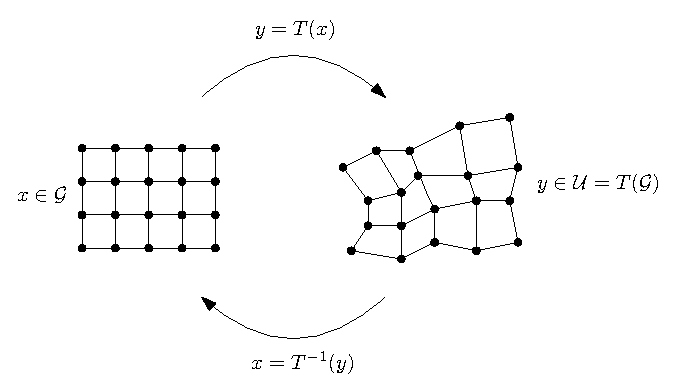
\includegraphics{grids.eps}
\end{center}

Let's solve the usual eikonal equation:
\begin{equation}
  \label{eq:eikonal}
  \|\nabla u(x)\| = s(x)
\end{equation}
on an unstructured grid of nodes $\mathcal{U} \subseteq \mathbb{R}^2$,
where we assume the nodes to be arranged into quadrilaterals with the
usual neighborhood connections. Let $\mathcal{G}$ be a regular grid
with the same number of nodes and topology as $\mathcal{U}$; denote
points in $\mathcal{G}$ by $x$ and points in $\mathcal{U}$ by $y$. Let
$T : \mathbb{R}^2 \to \mathbb{R}^2$ be a smooth vector field such that
$T(\mathcal{G}) = \mathcal{U}$ and such that it is locally invertible
at each $y \in \mathcal{U}$. Then:
\begin{equation}
  \| \nabla u(T^{-1}(y)) \| = s(T^{-1}(y)).
\end{equation}.
Since $\nabla (u \circ T^{-1}) (y) = \Jac_{T^{-1}}(y) \nabla u(T^{-1}(y))$, we can write this as:
\begin{equation}\label{eq:first-aniso}
  \| \Jac_{T^{-1}}^{-1}(y) \nabla (u \circ T^{-1}) (y) \| = (s \circ T^{-1})(y),
\end{equation}
since $T$ is locally invertible. Let $t(y) = (s \circ T)^{-1}(y)$,
$v(y) = (u \circ T^{-1}) (y)$, and $M(y) =
\Jac_{T^{-1}}^{-1}(y)/t(y)$. Then, \cref{eq:first-aniso} can be rewritten:
\begin{equation}
  \| M(y) \nabla v(y) \| = 1.
\end{equation}
Note that if $T(x) = y$ and $s > 0$, then:
\begin{equation}
  \frac{\Jac^{-1}_{T^{-1}}(y)}{t(y)} = \frac{\Jac_T(x)}{s(x)},
\end{equation}
by the inverse function theorem (may be useful for computations).

Maybe there are some errors in the above, but this seems intuitive:
solving an eikonal equation on an unstructured grid may be equivalent
to solving an anisotropic eikonal equation on a structured grid, and
vice versa: for an anisotropic eikonal equation with anisotropy
determined by $M : \mathbb{R}^2 \to \mathbb{R}^{2 \times 2}$, there
may be an unstructured grid on which the eikonal equation can
equivalently be solved.

\paragraph{Observations.}

\begin{itemize}
\item Starting with $\mathcal{U}$, deciding on $\mathcal{G}$, and
  finding $T$ is just an interpolation problem. Computing
  $\mathcal{G}$ from $\mathcal{U}$ might be slightly more tricky. The
  anisotropy $M(y)$ can be easily computed once $T$ is determined.
\item The inverse problem seems harder: starting with an arbitrary
  $M(y)$ and a structured grid $\mathcal{G}$, you would need to
  somehow ``smooth out'' the anisotropy and deform $\mathcal{G}$ into
  an unstructured grid $\mathcal{U}$ at the same time. I'm not sure
  how this would work exactly.
\end{itemize}

\paragraph{Questions.}

\begin{itemize}
\item Under what conditions is this possible?
\item What are the effects of different choices of $T$ on the accuracy
  of the solution?
\item 
\end{itemize}

\end{document}


%%% Local Variables:
%%% mode: latex
%%% TeX-master: t
%%% End:
